\documentclass[12pt,]{article}
\usepackage{lmodern}
\usepackage{amssymb,amsmath}
\usepackage{ifxetex,ifluatex}
\usepackage{fixltx2e} % provides \textsubscript
\ifnum 0\ifxetex 1\fi\ifluatex 1\fi=0 % if pdftex
  \usepackage[T1]{fontenc}
  \usepackage[utf8]{inputenc}
\else % if luatex or xelatex
  \ifxetex
    \usepackage{mathspec}
  \else
    \usepackage{fontspec}
  \fi
  \defaultfontfeatures{Ligatures=TeX,Scale=MatchLowercase}
\fi
% use upquote if available, for straight quotes in verbatim environments
\IfFileExists{upquote.sty}{\usepackage{upquote}}{}
% use microtype if available
\IfFileExists{microtype.sty}{%
\usepackage{microtype}
\UseMicrotypeSet[protrusion]{basicmath} % disable protrusion for tt fonts
}{}
\usepackage[margin=1in]{geometry}
\usepackage{hyperref}
\hypersetup{unicode=true,
            pdftitle={Incorporating dive behaviour into models of marine animal movement},
            pdfborder={0 0 0},
            breaklinks=true}
\urlstyle{same}  % don't use monospace font for urls
\usepackage{longtable,booktabs}
\usepackage{graphicx,grffile}
\makeatletter
\def\maxwidth{\ifdim\Gin@nat@width>\linewidth\linewidth\else\Gin@nat@width\fi}
\def\maxheight{\ifdim\Gin@nat@height>\textheight\textheight\else\Gin@nat@height\fi}
\makeatother
% Scale images if necessary, so that they will not overflow the page
% margins by default, and it is still possible to overwrite the defaults
% using explicit options in \includegraphics[width, height, ...]{}
\setkeys{Gin}{width=\maxwidth,height=\maxheight,keepaspectratio}
\IfFileExists{parskip.sty}{%
\usepackage{parskip}
}{% else
\setlength{\parindent}{0pt}
\setlength{\parskip}{6pt plus 2pt minus 1pt}
}
\setlength{\emergencystretch}{3em}  % prevent overfull lines
\providecommand{\tightlist}{%
  \setlength{\itemsep}{0pt}\setlength{\parskip}{0pt}}
\setcounter{secnumdepth}{5}
% Redefines (sub)paragraphs to behave more like sections
\ifx\paragraph\undefined\else
\let\oldparagraph\paragraph
\renewcommand{\paragraph}[1]{\oldparagraph{#1}\mbox{}}
\fi
\ifx\subparagraph\undefined\else
\let\oldsubparagraph\subparagraph
\renewcommand{\subparagraph}[1]{\oldsubparagraph{#1}\mbox{}}
\fi

%%% Use protect on footnotes to avoid problems with footnotes in titles
\let\rmarkdownfootnote\footnote%
\def\footnote{\protect\rmarkdownfootnote}

%%% Change title format to be more compact
\usepackage{titling}

% Create subtitle command for use in maketitle
\newcommand{\subtitle}[1]{
  \posttitle{
    \begin{center}\large#1\end{center}
    }
}

\setlength{\droptitle}{-2em}

  \title{Incorporating dive behaviour into models of marine animal movement}
    \pretitle{\vspace{\droptitle}\centering\huge}
  \posttitle{\par}
    \author{W. J. Grecian\(^1\)\footnote{Corresponding author:
  \href{mailto:james.grecian@gmail.com}{\nolinkurl{james.grecian@gmail.com}}}
, I. D. Jonsen\(^2\)\\
\(^1\)Sea Mammal Research Unit, Scottish Oceans Institute, University of
St Andrews\\
\(^2\)Dept. of Biological Sciences, Macquarie University, Sydney,
Australia}
    \preauthor{\centering\large\emph}
  \postauthor{\par}
      \predate{\centering\large\emph}
  \postdate{\par}
    \date{04 October 2018}

\usepackage{lineno}
\linenumbers
\usepackage{setspace}
\doublespacing

\begin{document}
\maketitle
\begin{abstract}
The Abstract must not exceed 350 words and should list the main results
and conclusions, using simple, factual, numbered statements.\\
1. Models of animal movement often only consider horizontal movement
over 2 dimensions. Incorporating vertical movement in these models
offers the potential to improve our understanding of the drivers of
animal movement.\\
2. Here we describe a state-space model that incorporates a random walk
on both horizontal and vertical movements, and estimates the covariance
between them. The model is flexible to allow both parameters to be
conditioned on covariates, offering insights into the drivers of animal
movement.\\
3. outline the main results\\
4. identify the conclusions and the wider implications.\\
\textbf{keywords:} A list in alphabetical order; not exceeding eight
words or short phrases; The most important key-words should appear in
the title; and the abstract; as well as the key-word list.
\end{abstract}

\begin{verbatim}
## Loading required package: citr
\end{verbatim}

\section{INTRODUCTION}\label{introduction}

Lorem ipsum dolor sit amet, est ad doctus eligendi scriptorem. Mel erat
falli ut. Feugiat legendos adipisci vix at, usu at laoreet argumentum
suscipiantur. An eos adhuc aliquip scriptorem, te adhuc dolor
liberavisse sea. Ponderum vivendum te nec, id agam brute disputando mei.

\section{MATERIALS AND METHODS}\label{materials-and-methods}

Lorem ipsum dolor sit amet, est ad doctus eligendi scriptorem. Mel erat
falli ut. Feugiat legendos adipisci vix at, usu at laoreet argumentum
suscipiantur. An eos adhuc aliquip scriptorem, te adhuc dolor
liberavisse sea. Ponderum vivendum te nec, id agam brute disputando mei.

\subsection{Equations}\label{equations}

The deterministic part of the model is defined by this \textbf{in-line
equation} as \(\mu_i = \beta_0 + \beta_1x\), and the stochastic part by
the \textbf{centered equation}:

\[ \frac{1}{\sqrt{2\pi}\sigma}e^{-(x-\mu_i)^2/(2\sigma^2)} \]

\subsection{Tables}\label{tables}

\begin{longtable}[]{@{}lrrrr@{}}
\caption{This is a GLM summary table.}\tabularnewline
\toprule
& Estimate & Std. Error & t value &
Pr(\textgreater{}\textbar{}t\textbar{})\tabularnewline
\midrule
\endfirsthead
\toprule
& Estimate & Std. Error & t value &
Pr(\textgreater{}\textbar{}t\textbar{})\tabularnewline
\midrule
\endhead
(Intercept) & -0.02 & 0.11 & -0.15 & 0.88\tabularnewline
x & 2.00 & 0.12 & 16.76 & 0.00\tabularnewline
\bottomrule
\end{longtable}

\subsection{Plots}\label{plots}

\begin{figure}[htbp]
\centering
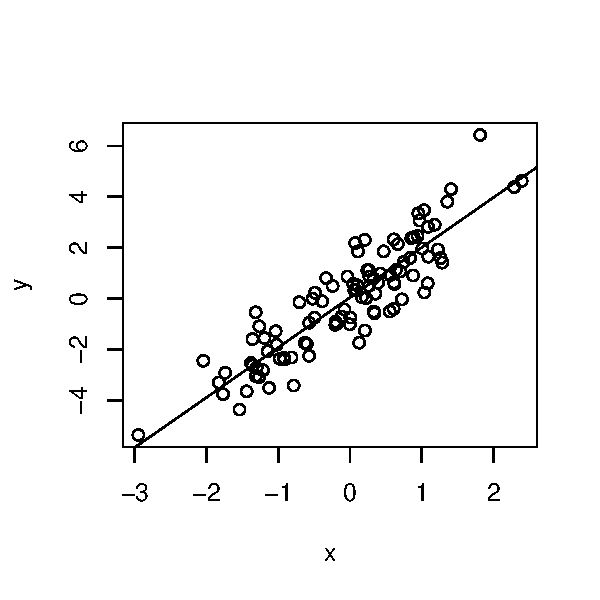
\includegraphics{manuscript_template_files/figure-latex/carDataPlot-1.pdf}
\caption{Relationship between x and y. The solid line is least-squares
linear regression.}
\end{figure}

\subsection{Citations}\label{citations}

The relationship was first described by Halpern, Regan, Possingham, \&
McCarthy (2006). However, there are also opinions that the relationship
is spurious (Keil, Belmaker, Wilson, Unitt, \& Jetz, 2012). We used R
for our calculations (R Core Team, 2016), and we used package.

\section{RESULTS}\label{results}

Lorem ipsum dolor sit amet, est ad doctus eligendi scriptorem. Mel erat
falli ut. Feugiat legendos adipisci vix at, usu at laoreet argumentum
suscipiantur. An eos adhuc aliquip scriptorem, te adhuc dolor
liberavisse sea. Ponderum vivendum te nec, id agam brute disputando mei.

\section{DISCUSSION}\label{discussion}

\section{CONCLUSION}\label{conclusion}

\section{ACKNOWLEDGEMENTS}\label{acknowledgements}

This project was made possible through a travel award from the Canada-UK
Foundation.

\section{AUTHORS' CONTRIBUTION}\label{authors-contribution}

\section{DATA ACCESSIBILITY}\label{data-accessibility}

\section*{REFERENCES}\label{references}
\addcontentsline{toc}{section}{REFERENCES}

\hypertarget{refs}{}
\hypertarget{ref-Halpern_2006}{}
Halpern, B. S., Regan, H. M., Possingham, H. P., \& McCarthy, M. A.
(2006). Accounting for uncertainty in marine reserve design.
\emph{Ecology Letters}, \emph{9}(1), 2--11.
doi:\href{https://doi.org/10.1111/j.1461-0248.2005.00827.x}{10.1111/j.1461-0248.2005.00827.x}

\hypertarget{ref-Keil_2012}{}
Keil, P., Belmaker, J., Wilson, A. M., Unitt, P., \& Jetz, W. (2012).
Downscaling of species distribution models: A hierarchical approach.
\emph{Methods in Ecology and Evolution}, \emph{4}(1), 82--94.
doi:\href{https://doi.org/10.1111/j.2041-210x.2012.00264.x}{10.1111/j.2041-210x.2012.00264.x}

\hypertarget{ref-R_Core_Team_2016}{}
R Core Team. (2016). \emph{R: A language and environment for statistical
computing}. Vienna, Austria: R Foundation for Statistical Computing.
Retrieved from \url{https://www.R-project.org/}


\end{document}
